\chapter{Uniform Linear Array}
In this section, we will be discussing a special case of arrays called the Uniform Linear array. From the previous section, we have studied the two element array and have seen how the three parameters, the ratio of the current amplitude $I_{2} / I_{1}$, the phase difference $\left(\delta_2 - \delta_1\right)$ and the inter-element spacing $d$ has a district effect on the radiation pattern. With this we will consider a more complex array which is the uniform linear array. It is important to note that in the case of the of the two element array, we had three (3) degrees of freedom but as the number of elements increases, the degree of freedom increases to $3(N -1)$ for $N$ elements and it allows for more flexibility. However, if we desire radiation in every specified direction, then spacing between the elements will not be a free parameter to control since it only increases the number of nulls and for lesser number of nulls we confine the spacing to fall between $\lambda/2$ and $\lambda$. Also we want direction of nulls and so the parameter $I_{2} / I_{1}$ is a constant unless there is need for complex form of radiation pattern. Therefore, the ratio of the current amplitude is not a free parameter. Finally when designing antenna arrays, we want control over the direction of the beam and so we vary the phase difference of the antenna elements. Also in designing array antennas, we do not require control of each and every antenna element, though it gives more flexibility, it requires complex electronic circuitry for controlling the phase of individual antennas and in many of the applications, it is not really required.

For the case of the uniform linear array, all elements are equally spaced, all elements are exacted with equal amplitude and the phase difference between adjacent elements is the same. So if the antenna elements are arranged along a straight line, uniformly, it is called a uniform linear array.
\begin{figure}
	\centering
	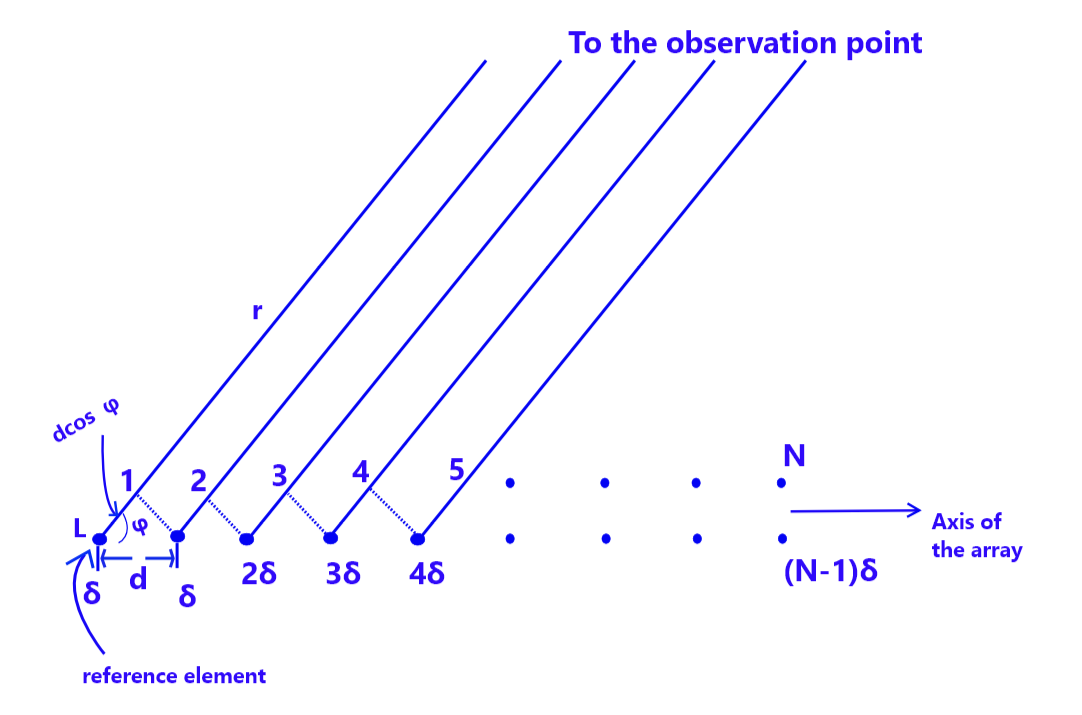
\includegraphics[height=5cm]{fig53_1}
	\caption{}
	\label{53.1}
	
\end{figure}

So let us examine $N$ element arrayed uniformly along a straight line as shown in Figure \ref{53.1}, that is, equally spaced. We assume the antenna element are isotropic in the plane and we will observe the radiation field at an observation point very far away which makes an angle of $\varphi$ with the array axis. The spacing between the elements is $d$ and the phase difference between two adjacent elements is $\delta$, so $\delta$ is the progressive phase shift. The amplitude of the currents in each element are the same and without losing generality, the amplitude $I$ would be unity.



Essentially for this array, there are three parameters we can control, they are: the phase shift $\delta$, the inter-element spacing $d$ and the number of elements $N$. If the reference element is a distance $r$ from the observation point,  then the next element will travel a distance $d\cos\varphi$ shorter and for the $N$th element, it would be $(N-1) d\cos\varphi $, which is the phase difference due to the arrangement. Therefore, the electric field can be written in terms of their magnitude and phase as follows:

\textbf{Note:} The total phase of each element is the sum of the space phase $(N-1) d\cos\varphi$ and the current phase $(N-1) \delta$.

\begin{align*}
&E_1 = E_0 e^{j0}\\
&E_2 = E_0 e^{j(\beta d\cos\varphi + \delta)} \\
&E_3 = E_0 e^{j2(\beta d\cos\varphi + \delta)} \cdots \\
&E_N = E_0 e^{j(N-1)(\beta d\cos\varphi + \delta)}
\end{align*}
where $$E_0 = \frac{kIe^{-j\beta r}}{r}$$ and let $$\psi = \beta d\cos\varphi + \delta$$ where $\beta d\cos\varphi$ is the space phase and $\delta$ is the electric phase.

The total electric field in the superposition of these fields at the observation point which is given as:

\begin{align*}
E &= E_1 + E_2 + E_3 + \dots + E_N \\
&= E_0e^{j0} + E_0e^{j\psi} + E_0e^{j2\psi} + \dots + E_0e^{j(N-1)\psi}
\end{align*}
\begin{equation}
\label{34}
E = E_0 \{1 + e^{j\psi} + e^{j2\psi} + \dots + e^{j(N-1)\psi} \}
\end{equation}
$1 + e^{j\psi} + e^{j2\psi} + \dots + e^{j(N-1)\psi}$ is the geometric series whose sum is given  as $$\frac{a(1-r^n)}{1-r}$$ where $a$ is the first term and $r$ is the common ratio and $n$ is the number of terms.

So,
$$
E = E_0 \left(\frac{1-e^{jN\psi}}{1-e^{j\psi}}\right) \quad \text{We rewrite the expression as:}
$$
$$
E = E_0 \frac{e^{j\frac{N\psi}{2}}}{e^{j\frac{\psi}{2}}} \left\{\frac{e^{-j\frac{N\psi}{2}} - e^{j\frac{N\psi}{2}}}{e^{-j\frac{\psi}{2}} - e^{j\frac{\psi}{2}}}\right\}
$$
Multiplying the numerator and denominator by $-1$, we have:
$$
E = E_0 \frac{e^{j\frac{N\psi}{2}}}{e^{j\frac{\psi}{2}}} \left\{\frac{e^{j\frac{N\psi}{2}} - e^{-j\frac{N\psi}{2}}}{e^{j\frac{\psi}{2}} - e^{-j\frac{\psi}{2}}}\right\}
$$

Recall that $e^{j\theta} - e^{-j\theta} = j2\sin\theta$, so
$$
E = E_0e^{j\frac{(N-1)\psi}{2}} \left\{\frac{\sin{\frac{N\psi}{2}}}{\sin{\frac{\psi}{2}}}\right\}
$$

Also, since we are interested in the radiation pattern then, 
\begin{equation}
\label{35}
\text{Radiation pattern} = \frac{1}{N} \frac{\sin{\frac{N\psi}{2}}}{\sin{\frac{\psi}{2}}}
\end{equation}
where $E_0$ is constant and $e^{j\frac{(N-1)\psi}{2}}$ is the phase term\footnote{Recall, 
	$$
	\text{Radiation pattern} = \frac{E(\theta, \varphi)}{E_{max}(\theta, \varphi)}
	$$
	Then the maximum electric field occurs when $\psi = 0$, that is the electric field in equation \ref{34} will add in phase to give $NE_0$ so dividing $E_0e^{j\frac{(N-1)\psi}{2}} \frac{\sin{\frac{N\psi}{2}}}{\sin{\frac{\psi}{2}}}$ by  $NE_0$ gives equation \ref{35} neglecting the phase $e^{j\frac{(N-1)\psi}{2}}$.
}.
The expression in equation \ref{35} shows that if the progressive space shift, the spacing between the elements and the total number of elements is known, then we can get the radiation pattern of the uniform array. 

So for the radiation pattern, we will examine the direction of maximum radiation, the direction of the nulls, the side lobe level and so on.

\section{Direction of Maximum Radiation ($\phi_{max}$)}
It is noted that at $\psi = 0$, there is maximum radiation. Also we will observe that when $\psi$ = multiples of $2\pi$, there will be maximum radiation. However, the direction which corresponds to $\psi = 0$ is the direction chosen. Normally, in designs, a specified direction is chosen and it is $\psi = 0$ which we recall is given as:
$$
\beta d\cos {\phi_{max}} + \delta = 0 
$$
$$
\text{where $\phi_{max}$ is the angle corresponding to maximum radiation}
$$
$$\phi_{max} = \cos^{-1}{(\frac{\delta}{\beta d})} \quad \text{for} \quad \beta = \frac{2\pi}{\lambda} $$
$$\phi_{max} = \cos^{-1}{(\frac{\delta \lambda}{2\pi d})}  $$
So by controlling the progressive phase shift, $\delta$ of the array thereby the direction of maximum radiation is known and then the value of $\delta$ can be gotten provided we choose a value for the inter-element spacing $d$ such that $\delta = -\beta \cos{\phi_{max}}$, then;
\begin{align}
\psi &=\beta d \cos {\varphi} + \delta \\
&=\beta d \cos{\phi} - \beta d \cos{\phi_{max}} \\
\label{36}
&=\beta d (\cos{\phi} - \cos{\phi_{max}}) \\
&=\frac{\lambda d}{2\pi}(\cos{\phi} - \cos{\phi_{max}})
\end{align}


Now the range of $\phi$ as we know goes from $0$ to $\pi$ so the value of $\phi_{max}$ will also go from $0$ to $\pi$.
There are two special cases for the antenna array which are the:
\begin{enumerate}
	\item [(a)] \textbf{End Fire array}: In this array, the maximum radiation is along the axis of the array. 
	\item[(b)] \textbf{Broadside array}: Here, the direction of maximum radiation is perpendicular to the axis of the array.
\end{enumerate}

Also for the end fire array $\phi_{max}$ is $\pi/2$. Therefore, the progressive phase shift for the end fire array given that $\delta = -\beta d\cos{\phi_{max}}$, $\phi_{max}=0$ or $\pi$ and $\cos{\phi_{max}} = \pm 1$ is $\delta = \pm \beta d$, so $\psi = \beta d \cos{\psi} + \delta = \beta d \cos{\psi} \pm \beta d $

Also for the broadside array, the progressive phase shift $\delta$ given that $\phi_{max} = \pi/2$ and so $\cos\phi_{max} = 0$ is $\delta = 0$, so $\psi = \beta d \cos{\phi}$. What this means for the broadside array is that all the currents are excited in phase ($\delta = 0$) and then all the radiation travels in the same direction corresponding to $\phi_{max} = \pi /2$. Figure \ref{53.2} shows the direction of maximum radiation for the two arrays. The radiation pattern of the end fire array can be said to be like that of an elongated balloon and that of the broadside array like a flattened disc.

\begin{figure}
	\centering
	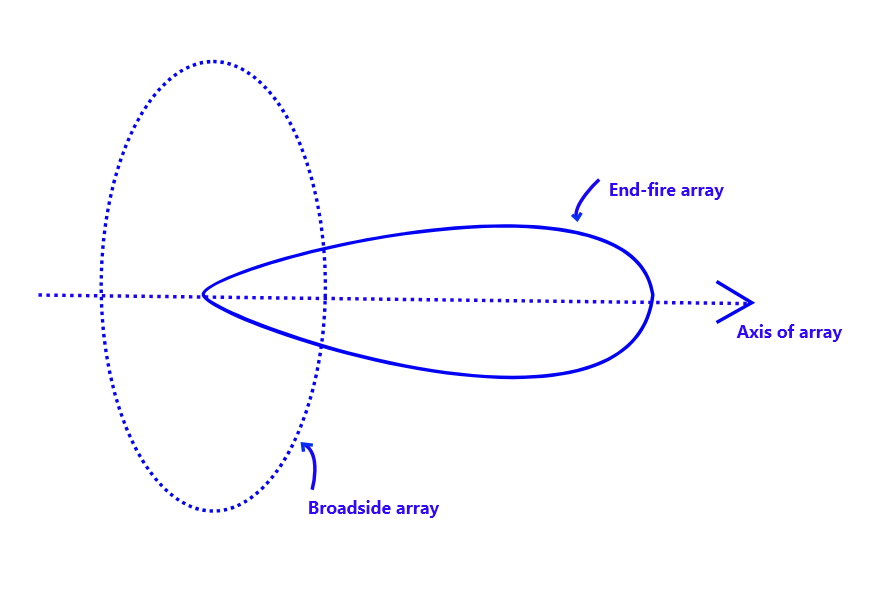
\includegraphics[width=8cm]{fig53_2}
	\caption{Radiation patterns of the two special cases}
	\label{53.2}
	
\end{figure}


\section{Direction of Nulls}
From the radiation pattern given as $\frac{1}{N} \frac{\sin{\frac{N\psi}{2}}}{\sin{\frac{\psi}{2}}} $ we have sine function of $\psi$ and a large value of $N$ the numerator $\sin{\frac{N\psi}{2}} $ will have a large frequency. Figure \ref{53.3} shows the plot of the modulus of $\sin{\frac{N\psi}{2}}$ and $\sin{\frac{\psi}{2}}$ as that $\psi$ varies from $0$ to $2\pi$. Essential two things can be observed. 

\begin{enumerate}
	\item [(1)] Whenever $\arrowvert \sin{\frac{N\psi}{2}} \arrowvert$ goes to zero the radiation field will go to zero 
	\item [(2)] Whenever $\arrowvert \sin{\frac{N\psi}{2}} \arrowvert$ goes to maximum since $\arrowvert \sin{\frac{\psi}{2}} \arrowvert$ is a slow varying function, it would correspond to a local maximum and it gives the magnitude of the side lobes.
\end{enumerate}




\begin{figure}
	\centering
	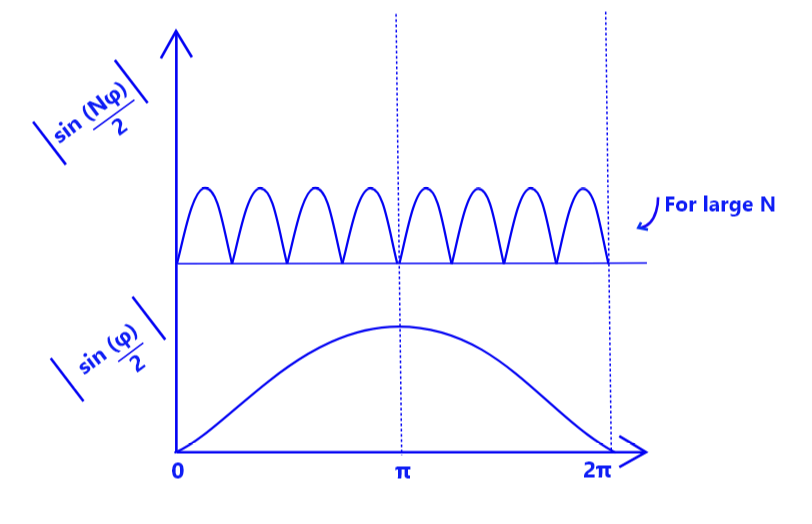
\includegraphics[height=5cm]{fig53_3}
	\caption{}
	\label{53.3}
	
\end{figure}


So, $\sin{\frac{N\psi}{2}}$ decides the direction of nulls as well as the deviation of the side lobes. Therefore, for the direction of nulls
$$\sin{\frac{N\psi}{2}} = 0$$
That is when  $\frac{N\psi}{2} = \pm m \pi$ where $m=1,2,3, \cdots \quad \footnote{ At $m=0$, it corresponds to $\phi = 0$ which is the direction of maximum radiation}$ 

From Equation \ref{36}, 
$$ \psi  =  \beta d \{\cos{\phi_{null}} -\cos{\phi_{max} } \} = \pm \frac{2m\pi}{N}$$
Where $\phi_{null}$ denotes the direction of a null
$$\cos{\phi_{null}} -\cos{\phi_{max} }  = \pm \frac{2m\pi}{N\beta d}$$
$$\cos{\phi_{null}} = \cos{\phi_{max} }  \pm \frac{2m\pi}{N\beta d} $$
$$\cos{\phi_{null}} = \cos{\phi_{max} }  \pm \frac{m\lambda}{Nd} \quad \text{since $\beta = \frac{2\pi}{\lambda}$} $$

Therefore, once the direction of maximum radiation $\phi_{max}$ is known, the direction of element $N$ is known and the spacing between the antenna element $d$ is known, we can find out the directions of nulls. It should be noted that the values of null should lie in the visible region where $\phi$ ranges from $0$ to $\pi$ or $\cos{\phi}$ ranges from $-1$ to $+1$. Also, we should note that when $N$ is very large, there are more numbers for $m$ which will cause $\cos{\phi}$ to fall within the range of $-1$ to $+1$  and it means more nulls for the same inter-element spacing $d$. So as we increase the number of elements, the number of nulls increases which implies more side lobes.

Now lets consider a case study where the direction of maximum $\phi_{max} = 0$. So that $\cos{\phi} = \cos{\phi_{max}} \pm \frac{m\lambda}{N d}$ becomes:
$$\cos{\phi} = 1 \pm \frac{m\lambda}{N d} \quad \text{and so in this case $m=1,2,3, \cdots$} $$
because at $m=0$, we have $\phi_{max}$ so the nulls will be given by other values of $m$. Since $\cos{\phi}$ should lie between $+1$ and $-1$ then:
$$\cos{\phi} = 1 - \frac{m \lambda}{N d} \quad \text{for $m=1, 2,3,\cdots$}$$

It should be noted that given $\psi = \pm \frac{2m\pi}{N}$ where $m$ varies to whatever value permissible for the nulls, the nulls will be equally spaced in  $\psi$ domain by a spacing of $\frac{2\pi}{N}$ but due to the non-linear relationship between $\psi$ and $\phi$, that is $\psi \propto \cos{\phi}$, the nulls are bit equally spaced in the physical space. Also we know that there is a side lobe between every two nulls so when $\sin{\frac{N\psi}{2}} = 1$ or $\frac{N\psi}{2} = $ odd multiples of $\frac{\pi}{2}$, there would be a side lobe. In the $\psi$ domain half way between every nulls there is a maximum (side lobe) so we can say approximately in the physical space that there is the side lobe.


\section{Direction of the Side Lobe ($\phi_{SL}$)}
We earlier said that the local maximum (side lobe ) is given by the function $\sin{(\frac{N\psi}{2})}$ so when $\sin{(\frac{N\psi}{2})} = 1$ gives the side lobes, therefore, 
$$ \frac{N\psi}{2} \quad = \quad \text{odd multiples of $\pi/2$} \quad = \quad \pm (m + 1/2) \pi $$
Substituting $ \psi = \beta d (\cos\phi - \cos\phi_{max}) $ gives:
$$ \psi = \beta d (\cos\phi_{SL} - \cos\phi_{max}) \quad= \quad \pm \frac{2(m + 1/2) \pi}{N}$$
where $\phi_{SL}$ in the direction of the side lobes:
$$ \cos\phi_{SL} - \cos\phi_{max} \quad= \quad \pm \frac{2(m + 1/2) \pi}{N \beta d} $$
$$ \cos\phi_{SL} \quad= \quad  \cos\phi_{max}  \quad \pm \quad \frac{2(m + 1/2) \pi}{N \beta d} $$

$$ \cos\phi_{SL} \quad= \quad  \cos\phi_{max}  \quad \pm \quad (m + 1/2) \frac{\lambda}{dN} \quad \text{ since $\beta=\frac{2\pi}{\lambda}$} $$

Again, we will choose the values of $m$ such that $\cos\phi_{SL}$ lies between $-1$ and $+1$ and the direction $\phi_{SL}$ will represent the direction of the side lobes. One might argue that the direction of the side lobe should be given by differentiating the expression $\sin{(\frac{N\psi}{2})}$. However, following, the simple logic that says that in between every two nulls, there is a maximum makes it very easy to calculate the directions of the side lobes. So basically, we have a side lobe that is approximately halfway between the nulls in physical space.

\section{Side Lobe level of the array}
This is an important parameter because it shows how much energy is leaked in the direction in which we never intended to send energy. Now we know the directions of the side lobes which is when $\frac{N\psi}{2} = \pm (m + 1/2) \pi $ for $m=1,2,3,\cdots$. Notice that $m$ start counting from $1$, this is because the first side lobe will occur after the first null  (at $\frac{N\psi}{2} = \pi$). So substituting in %CHECK
we will get the values of $\frac{N\psi}{2}$ for the first, second, third side lobes and so on.\\

\textbf{First side lobe:}
$$\frac{N\psi}{2} = \frac{3\pi}{2} \quad \text{for $m=1$} $$
$$ \frac{\psi}{2} = \frac{3\pi}{N2} $$

Amplitude of the first side lobe is given by substituting $\frac{\psi}{2}$ in the radiation pattern expression, that is
$$\frac{1}{N} \frac{\sin{\frac{N\psi}{2}}}{\sin{\frac{\psi}{2}}} = \frac{1}{N} |{\frac{1}{\sin{\frac{3\pi}{2N}}} |}   $$
If $N$ is extremely large, then $\sin{(\frac{3\pi}{2N})} \approx  \frac{3\pi}{2N}$, then the amplitude is given as $$\approx \frac{2}{3\pi}$$


\textbf{Second side lobe:}
$$\frac{N\psi}{2} = \frac{5\pi}{2N} \quad \text{for $m=2$} $$

So amplitude of the second side lobe  $\approx \frac{2}{5\pi}$ and the amplitude of the third side lobe is $\approx \frac{2}{7\pi}$ and so on. A plot of the radiation pattern along the $\psi$ axis is shown in Figure \ref{53.4}, showing the linear relationship and polar relationship.

\begin{figure}
	\centering
	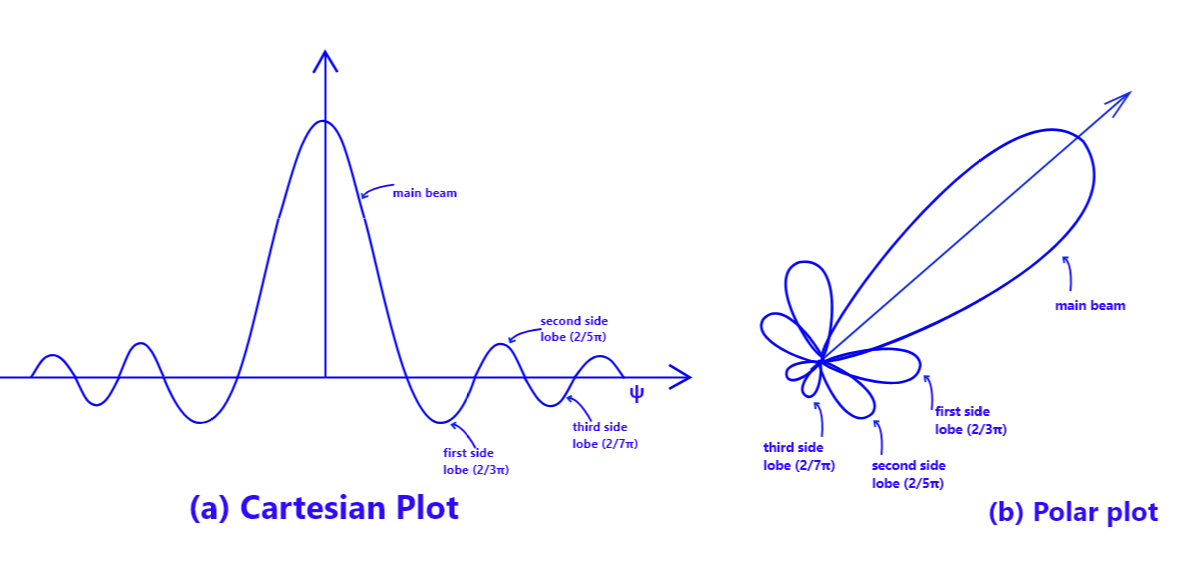
\includegraphics[width=1\linewidth]{fig53_4}
	\caption{}
	\label{53.4}
	
\end{figure}


It is observed that as we move away from the main beam,  the amplitude goes on decreasing so the highest side lobe is essentially the first side lobe. The side lobe level of the side lobes are given as the amplitude of the side lobe divided by the amplitude of the main beam (which is $1$). So for the first lobe, the side lobe level is $21\%$, for the second lobe, the side lobe level is $13\%$ and so on. It is important to note that the level of side lobe (side lobe level) is not dependent on any of the array parameter, that is, the inter-element spacing, the number of elements, and the phase shift. However, the progressive phase shift controls the direction of the maximum radiation and the number of elements controls the number of nulls but the amplitude of the side lobe is independent of the number of elements. As long as $N$ is large enough. The side lobe $21\%$ which essentially means that for the uniform array, there is power leak  from each side lobe of about $21\%$, $13\%$ and so on, starting from the first side lobe and if it is summed up, the total substantial loss in the directions of the side lobes compared to the main beam is gotten.